\begin{figure}
    \centering
    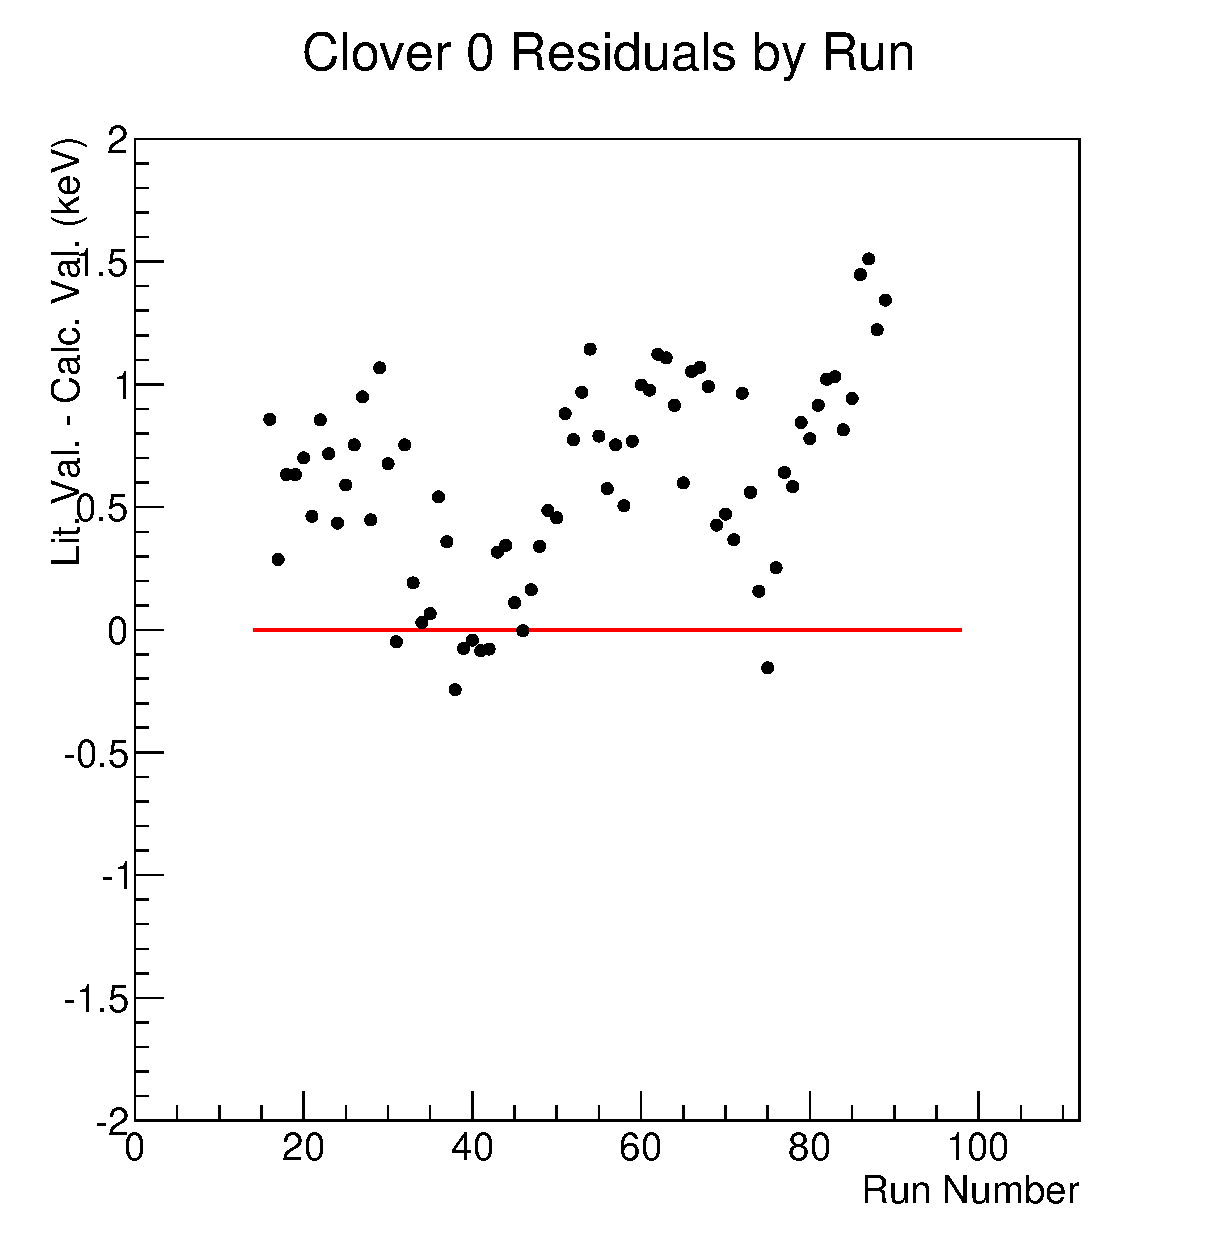
\includegraphics[scale=0.6]{Analysis_Figs/residual_by_run.eps}
    \caption[Example of calibration drift by run.]{The difference between the literature value and the calibrated value (before run-by-run correction) of the naturally occurring $^{40}$K background peak at 1460 keV, plotted by run for one leaf of one HPGe detector. The red line shows $\Delta E=0$.}
    \label{fig:clover_run}
\end{figure}